\documentclass[fontsize=10pt,paper=a4,bibliography=totoc]{scrartcl}

\usepackage[utf8]{inputenc}
\usepackage[ngerman]{babel}
\usepackage{amsmath}
\usepackage{graphicx}
\usepackage{units}
\usepackage{url}
\title{Ausarbeitung\\Solarthermisches Kraftwerk}
\author{K. Franke, M. Dolgov, F. Achilles}
\begin{document}
\maketitle

\section{Stand der Technik}
\subsection{Dish-Stirling Anlage}
Die Dish-Stirling Anlage besteht aus einem großen Parabolspiegel, der meistens aus mehreren kleinen Spiegeln zusammengesetzt wird. Im Brennpunkt befindet sich ein Stirling Motor, der aus der gebündelten Wärme Strom erzeugt. Damit die Strahlen sich immer im Brennpunkt treffen, wird der große Parabolspiegel mit der Sonne mitgedreht um immer senkrecht einfallende Strahlen zu erreichen. Für dieses Konzept ist somit immer eine zweiachsige Nachführung des Spiegels nötig, da nicht senkrecht einfallende Strahlen den Absorber des Stirling Motors verfehlen würden. Dieses Konzept funktioniert daher nur bei direkter Sonneneinstrahlung und nicht bei diffusem Licht. Bild einfügen! Vorteil dieses Kraftwerktyps ist die sehr kompakte Bauweise, so können diese Kraftwerke schon für Leistungen ab ??
%TODO Finden
 kW eingesetzt werden. Nachteil ist die Skalierbarkeit. So kann die Spiegelgröße zwar nach der geforderten Leistung und der Sonneneinstrahlung am Standort gewählt werden, dies ist konstruktionsbedingt aber nur bis zu einer gewissen Größe möglich, da die Windlasten des Spiegels immer größer werden. Besonders die Nachführung wird bei steigender Spiegelgröße immer größer und damit teurer.
 
\subsection{Parabolrinnenkraftwerk}
Das Parabolrinnenkraftwerk fokussiert die einfallenden Strahlen nicht auf einen Punkt, sondern auf eine meist mit Öl gefüllte, im Brennpunkt liegende Röhre. Da es sich hier nicht um einen Punktabsorber, sondern um einen in eine Dimension ausgebreiteten Absorber handelt, ist auch nur eine eindimensionale Nachführung nötig. Das erhitzte Öl kann anschließend über Wärmetauscher in einem Gas und Dampfkraftwerk Strom erzeugen. Bild einfügen! Vorteil dieser Technik im Vergleich zur Dish-Stirling Anlage ist, dass eine einachsige Nachführung günstiger ist und das System sehr gut skaliert. Außerdem ist durch ein stationäres Kraftwerk ein besserer Wirkungsgrad erreichbar als durch einen Stirlingmotor
%TODO Nachweis für Wirkungsgrad
 (Nachweis einfügen, wer findet einen?). In großen Solarthermiekraftwerken werden daher meistens Parabolrinnen eingesetzt. Nachteil ist, dass hier eine größere Fläche nötig ist, damit sich der Bau eines stationären Kraftwerks lohnt.
\emph{Gesamtwirkungsgrad hinzufügen wenn ihn jemand findet, vielleicht auch rauslassen, wenn wir den Gesamtwirkungsgrad von unserem Kraftwerk nicht berechnen können.}
\section{Idee}
Ziel dieses Projekts ist die Kombination der kompakten Bauweise einer Dish-Stirling Anlage und der guten Skalierbarkeit des Parabolrinnenkraftwerks mit ein stationären Kraftwerk. Da das Kraftwerk für den Standort Karlsruhe entwickelt werden soll, ist auch zu bedenken, dass hier auch sehr viel diffuse Sonnenstrahlung vorhanden ist, die nach Möglichkeit genutzt werden sollte. Aufgrund der kleinen Abmessungen von nur $10\unit{m}^3$ kam nur eine zweidimensionale Nachführung in Kombination mit einem großen Parabolspiegel in Frage, dabei sollte aber der große Spiegel wegen der Windlasten und einer deutlich einfacheren Konstruktion nicht nachgeführt werden. Stattdessen wurde ein zweiter, deutlich kleinerer Spiegel hinzugefügt, der zweiachsig auf einer Schiene nachgeführt wird und immer im Fokuspunkt der Strahlen steht. Dieser Spiegel reflektiert die eingefangenen Strahlen wieder zurück auf die Mitte des großen Spiegels wo der Absorber platziert ist. Das einzig bewegliche Teil ist also ein leichter Spiegel, der auf einer Schiene fährt. Der Absorber kann wie im Fall des Parabolrinnenkraftwerks an ein stationäres Kraftwerk gekoppelt werden, es entfällt aber der Transport des Öls. Da sich ein Gas und Dampfkraftwerk bei der gegebenen Grundfläche nicht rentiert, wird ein alternatives Konzept vorgeschlagen, das durch die Erwärmung von Luft eine Druckdifferenz erzeugt, die über einen Luftdruckmotor in elektrischen Strom gewandelt werden kann.

\section{Vorstellung des Konzepts}
Es wurde zuerst untersucht wie sich schräg einfallende Strahlung auf den Fokuspunkt der Strahlen auswirkt. Für solche Versuche wurde ein Raytracing Programm in Matlab geschrieben, das beliebig viele Strahlen in einer beliebigen Richtung erzeugt, den Schnittpunkt mit einem Spiegel findet, die Reflexionsrichtung berechnet und alles grafisch darstellen kann. Das Ergebnis ist in Abbildung~\ref{pic:2dreflektion} zu sehen. Während die Strahlen bei senkrechtem Lichteinfall genau im Fokuspunkt gebündelt werden, verschiebt sich dieser
bei schrägem Einfall%hat gefehlt ;)
nicht nur, die Strahlen werden nun auch nicht mehr so gut gebündelt, sondern fächern auf (siehe Abbildung~\ref{pic:2dreflektion_schraeg}). 

\begin{figure}[htb]
	\centering
	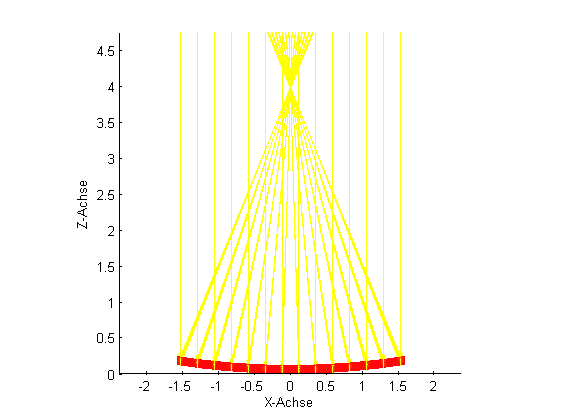
\includegraphics[width=\textwidth]{images/2d_gerade}
	\caption{Gerader Einfall auf Parabolspiegel}
	\label{pic:2dreflektion}
\end{figure}
\begin{figure}[htb]
	\centering
	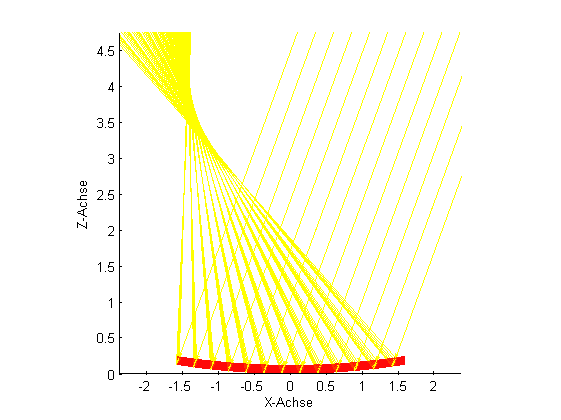
\includegraphics[width=\textwidth]{images/2d_schraeg_20_grad}
	\caption{Schräger Einfall auf Parabolspiegel (20$^{\circ}$ zur vertikalen Achse)}
	\label{pic:2dreflektion_schraeg}
\end{figure}

\subsection{Erhoffte Vorteile}

\section{Beschreibung des Programms}
\subsection{Ablaufdiagramm (Top-Level)}
\subsection{Möglichkeiten und Grenzen}
 (versch. Breitengrade, über ein Jahr hinweg etc.)
\section{Gesamtaufbau}
\subsection{CAD-Modell mit allen Nebenaggregaten}
 (Antriebe: Stirling, Turbine)
\subsection{Verschiedene Generatorantriebe}
 (Stirling, Turbine)
\section{Kosten}
\section{Ergebnisse}


\section{Alles Mögliche}

\begin{align*}
	AirMass(\xi)=\frac{1}{\cos(\xi)}
\end{align*}

\begin{figure}[htb]
	\centering
	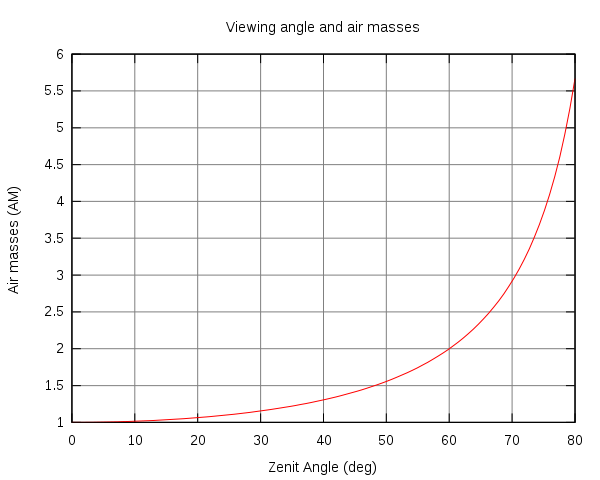
\includegraphics[width=\textwidth]{images/Airmass.png}
	\caption{Luftmasse in Abhängigkeit vom Zenit-Winkel}
	\label{pic:AirMass}
\end{figure}

\begin{table}
\centering
	\caption{Werte für Strahlungsleistung. Wiki (engl) air mass solar energy. Stand 08.06.}
	\label{tab:airmass}
\begin{tabular}{|c|c|c|}
	\hline
	$\alpha$ & Air Mass & $\frac{W}{m^2}$\\
	\hline
	- & 0 & 1367\\
	\hline
	0 & 1 & 1040\\
	\hline
	23 & 1.09 & 1020\\
	\hline
	48.2 & 1.5 & 930\\
	\hline
	75 & 3.8 & 620\\
	\hline
	85 & 10 & 270\\
	\hline
\end{tabular}
\end{table}
Test
\begin{align*}
	I=1,1\cdot I_0 \cdot 0,7^{AM^{0,678}}
	\label{eqn:Intensity}
\end{align*}

Wir sollten die Quellen mit BibTex organisieren, welches Programm nehmt ihr da? Ich kenn nur BibDesk aus dem IBT, werd das mal suchen.

Quellen:

\url{http://www.fvee.de/fileadmin/publikationen/Themenhefte/th2002/th2002_02_03.pdf}
\end{document}
